\documentclass[aspectratio=169]{beamer}

\usepackage{xltxtra}
\usepackage[main=russian,english]{babel}
\defaultfontfeatures{Mapping=tex-text}
\usepackage{listings}

\usepackage[backend=biber,bibstyle=numeric,citestyle=numeric-comp,sorting=none,defernumbers=true,date=long]{biblatex}
\addbibresource{strangego.bib}

\makeatletter
\let\old@lstKV@SwitchCases\lstKV@SwitchCases
\def\lstKV@SwitchCases#1#2#3{}
\makeatother
\usepackage{lstlinebgrd}
\makeatletter
\let\lstKV@SwitchCases\old@lstKV@SwitchCases

\lst@Key{numbers}{none}{%
    \def\lst@PlaceNumber{\lst@linebgrd}%
    \lstKV@SwitchCases{#1}%
    {none:\\%
     left:\def\lst@PlaceNumber{\llap{\normalfont
                \lst@numberstyle{\thelstnumber}\kern\lst@numbersep}\lst@linebgrd}\\%
     right:\def\lst@PlaceNumber{\rlap{\normalfont
                \kern\linewidth \kern\lst@numbersep
                \lst@numberstyle{\thelstnumber}}\lst@linebgrd}%
    }{\PackageError{Listings}{Numbers #1 unknown}\@ehc}}
\makeatother

\setmainfont{Arial}

\title{Код Хэмминга}
\author{Тронин Олег Александрович}

\usetheme{gcr2019}


\setbeamercolor{itemize item}{fg=text}
\setbeamercolor{itemize subitem}{fg=text}
\setbeamercolor{alerted text}{fg=text}
\setbeamertemplate{itemize items}{\textbullet}
\setbeamerfont*{itemize/enumerate subbody}{parent=itemize/enumerate body}
\setbeamerfont*{itemize/enumerate subsubbody}{parent=itemize/enumerate subbody}
\setbeamerfont{alerted text}{series=\bfseries}

\definecolor{acmebg}{HTML}{FFFFEF}
\definecolor{acmeh}{HTML}{EFFFFF}
\definecolor{acmec}{HTML}{8C8ACE}
\definecolor{acmel}{HTML}{52AAAD}
\definecolor{acmel1}{HTML}{EFEF9C}
\definecolor{acmel2}{HTML}{9CEFEF}
\lstset{
        columns=flexible,
        keepspaces=true,
        showstringspaces=false,
        showtabs=false,
        tabsize=4,
        frame=single,
        basicstyle=\fontsize{10pt}{12}\bf\ttfamily\color{black},
        backgroundcolor=\color{acmebg},
        commentstyle=\color{black},
        keywordstyle=\color{black},
        stringstyle=\color{red},
        rulecolor=\color{acmel},
        framerule=1pt
}

\setbeamerfont{bibliography item}{size*={8pt}{1}}

\setbeamertemplate{bibliography item}{\insertbiblabel}
\renewcommand*{\bibfont}{\fontsize{8}{1}\selectfont}
\DeclareFieldFormat{url}{\color{blue}\url{#1}}


\newcommand{\clbox}[2]{%
  \hspace*{-\fboxsep}\colorbox{#1}{#2}\hspace*{-\fboxsep}%
}

\makeatletter

\newcount\bt@rangea
\newcount\bt@rangeb

\newcommand\btIfInRange[2]{%
    \global\let\bt@inrange\@secondoftwo%
    \edef\bt@rangelist{#2}%
    \foreach \range in \bt@rangelist {%
        \afterassignment\bt@getrangeb%
        \bt@rangea=0\range\relax%
        \pgfmathtruncatemacro\result{ ( #1 >= \bt@rangea) && (#1 <= \bt@rangeb) }%
        \ifnum\result=1\relax%
            \breakforeach%
            \global\let\bt@inrange\@firstoftwo%
        \fi%
    }%
    \bt@inrange%
}
\newcommand\bt@getrangeb{%
    \@ifnextchar\relax%
        {\bt@rangeb=\bt@rangea}%
        {\@getrangeb}%
}
\def\@getrangeb-#1\relax{%
    \ifx\relax#1\relax%
        \bt@rangeb=100000% 
    \else%
        \bt@rangeb=#1\relax%
    \fi%
}

\newcommand<>{\btLstHL}[1]{%
\only#2{\btIfInRange{\value{lstnumber}}{#1}{\color{acmel1}\def\lst@linebgrdcmd{\color@block}}{\def\lst@linebgrdcmd####1####2####3{}}}%
}%
\makeatother

\begin{document}

\begin{frame}
\titlepage
\end{frame}

\begin{frame}{Формулировка задачи}
Рассмотрим четыре круга, пересекающиеся так, как показано на рисунке. Назовём лепестком каждую из трёх фигур, образованных пересечением трёх кругов.
Запишем в каждом из кругов ноль или единицу. После этого в каждом лепестке запишем остаток при делении на два суммы чисел во всех кругах, в которых содержится этот лепесток. Например, если в кругах были записаны числа 0, 1, 0, 1, то в лепестках будут записаны числа 0, 1, 0 (круги и лепестки перечислены в порядке, указанном на рисунке).
\end{frame}

\begin{frame}
Описанная схема называется кодом Хэмминга и обладает интересным свойством. Если ваш враг в тайне от вас изменит любое из семи записанных по этой схеме чисел, вы сможете однозначно определить, какое число он изменил. Решив эту задачу, вы узнаете, как это сделать.
\end{frame}

\begin{frame}{Условия задачи}
     
		\begin{itemize}
                		\item Исходные данные:
В единственной строке через пробел записаны семь чисел. Каждое из чисел равно нулю или единице. Сперва идут четыре числа, записанные в кругах в порядке, указанном на рисунке. Далее идут три числа, записанные в лепестках в порядке, указанном на рисунке.:
        \end{itemize}

\end{frame}

\begin{frame}
	\begin{columns}[T,onlytextwidth]
                        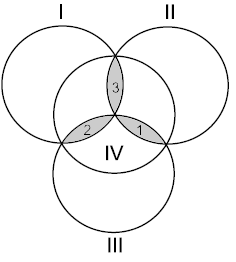
\includegraphics[width=0.54\textwidth]{acme-alef.png}
        \end{columns}
\end{frame}

\begin{frame}
        \begin{itemize}
                \item Результат
В единственной строке выведите через пробел семь чисел, образующие код Хэмминга. Набор чисел должен отличаться от исходного не более чем в одном числе. Гарантируется, что любой набор входных данных либо сам является кодом Хэмминга, либо в нём можно изменить в точности одну цифру и получить код Хэмминга.
        \end{itemize}
\end{frame}

\begin{frame}{Решение задачи}
        \textbf{Так как на вход мы получаем семь цифр,состоящих из нулей и единиц. При этом первые четыре цифры это условие, оставшиеся три это результат. Нам достаточно проверить что бы при сложении по модулю два, первой, второй, и четвёртой мы получили число которое стоит на позиции пять, тоже самое для цифр на первой, третьей и четвертой соответствует результат на шетой позиции, и для цифр на второй, третьей и четвёртой - цифра на седьмой позиции.}
\end{frame}

\begin{frame}
        \textbf{Так как в условии задачи сказано что необходимо изменить одно и только одно число, то самый простой способ это перебор всех цифр подряд, то есть мы просто меняем первую цифру на противоположную и снова проверяем изначальное условие, если ответ утвердителен, код найден, в противном случае возвращаем значение первой цифры и меняем уже вторую, и так мы делаем до самой последней цифры, когда она поменяется в значении, мы получим положительный ответ и найдём код Хэмминга.}
\end{frame}

\begin{frame}{Код программы}
        \begin{columns}[T,onlytextwidth]
                        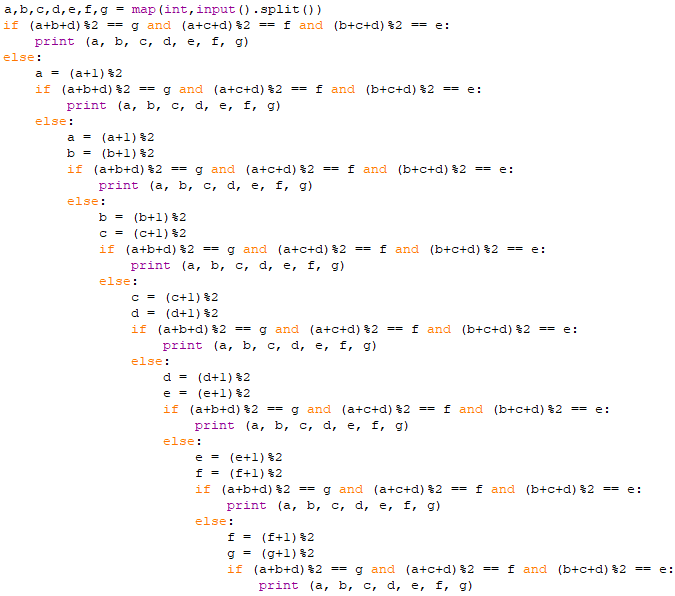
\includegraphics[width=0.82\textwidth]{Hemming.png}
        \end{columns}
\end{frame}

\begin{frame}
        \begin{columns}[T,onlytextwidth]
                        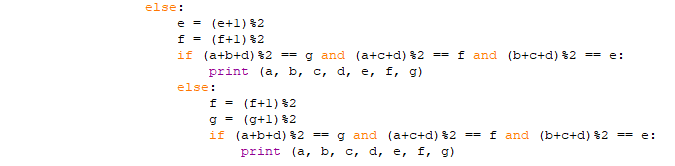
\includegraphics[width=0.82\textwidth]{Hemming2.png}
        \end{columns}
\end{frame}

\end{document}

